\documentclass[11pt]{article}
\usepackage{common}

\usepackage{float}
\usepackage{graphicx}
\title{CS 182 Final Project: \\ Building A Backgammon AI}
\author{Virgile Audi \\ vaudi@g.harvard.edu}
\begin{document}
\maketitle{}


\section{Introduction}

Backgammon is one of the oldest board game known to man. We can trace back its origins to Ancient Egypt, dating back 3500 BC, and most of the neighbouring empires had their own version of what resembles today Backgammon. Backgammon is a two player zero-sum game where the objective is to removing all of one's pawns before his opponent. Players move their pawns according to the roll of two dice. It is therefore both a game of strategy and luck (which we will see will impact the use of certain algorithms). It is said that learning to play backgammon is relatively easy, but learning to play backgammon well is extremely hard. The goal of this project was to build an AI capable of playing backgammon. The methodology was inspired by DeepMind's work on Alpha Go. To simplify, the methodology I decided to use, and for which I have not been able to find similar work in the backgammon literature, is to first used supervised learning in the form a multiclass logistic regression as the initial state of reinforcement learning using genetic algorithms and Q-learning. 

\begin{figure}[H]
\begin{center}
    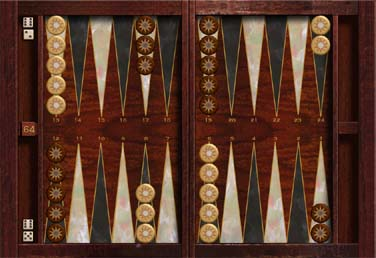
\includegraphics[width=0.6\textwidth]{board.jpg}
\end{center}
\caption{Backgammon Board}
\end{figure}

\section{Background and Related Work}

The literature is mainly dominated by the work of Gerald Tesauro who developped TD-Gammon in 1992 \cite{tdg}. His AI, which is still considered one of the best (if not the best) in the backgammon sphere, consists of a neural network trained using TD-($\lambda$). I tried to stay away of Neural Networks as this was not the focus of this class and sticked to linear evaluation functions. As mentioned in the introduction, I was inspired by the work on "AlphaGo" \cite{alpha}. I was interested to see how much of a head start would supervised learning could give reinforcement learning, and hopefully compensate for the use of linear functions instead of neural nets. For the reinforcement learning part of this project, I adapted methods from two papers. The first one \cite{expert} presented encouraging results of the use of TD learning where the AI would face an already trained opponent, contrary to TD-Gammon where the AI would face himself. The second paper \cite{genetic} showed how we could use a certain type of genetic algorithm, which will be presented in the following sections, to update the weights of the evaluation function. Nevertheless, both of these methods were originally presented in the context of uninformed reinforcement learning i.e. where the initial weights of the evaluation function are initialised randomly. I, on the contrary, adapted these methods (some with success, some without unfortunately) by initialising these algorithms using the results of the supervised learning from expert moves. 
 

\section{Problem Specification}
In order to explain formally how the problem was formulated mathematically, a few basic rules of backgammon should be explained.
\subsection{Backgammon's Rules}
In the introduction, I mentioned that the goal of backgammon was to remove all of ones pawns before his/her opponent according to the rolls of two dice but this is still pretty vague. Let's dig into more details. Each player needs to first bring every pawns of his into his camp which following the directions of the white and red arrows below on figure 2. Let's showcase a example. Consider the white player rolls (6,5), he can effectively move any pawn in the direction of the white arrow 6 or 5 position forward. A move is acceptable for the white player if the destination is either empty (no pawns white or black are present), already occupied by one or more white pawns or if only one black pawn is occupying the space. In this last case, the white player captures his opponents pawn, who will then need to free his pawn in his oppenent camp. Figure 3 shows for instance the possible moves for the white player when rolling (6,5).\\

\noindent Backgammon can therefore been seen as a succession of boards and rolls of dice. The problem that therefore needs to be solved is to which board should one player move to given the current board and the roll of the dice. How can we evaluate the boards so that the player can move to the board with the highest value?

\begin{figure}[H]
\centering
\begin{minipage}{.35\textwidth}
  \centering
  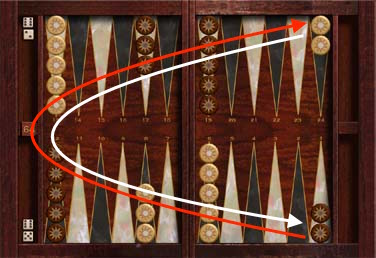
\includegraphics[width=0.75\linewidth]{board_general.jpg}
  \caption{General Dynamics}
\end{minipage}%
\begin{minipage}{.35\textwidth}
  \centering
  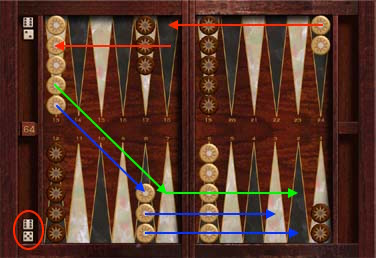
\includegraphics[width=0.75\linewidth]{moves.jpg}
  \caption{Possible Moves}
\end{minipage}
\end{figure}

\subsection{Formal Description}

If we define the states to be a tuple (board, roll) and action be the possible moves given the board and the roll, then Backgammon fits perfectly in the litterature of Markov Decision Process. Formally:
\begin{itemize}
\item Let $s = (b, r) \in \mathcal{S} = \mathcal{B}\times\mathcal{R}$ be the states
\item Let $a \in \mathcal{A}$ with $a: s\rightarrow b \in \mathcal{B}$
\end{itemize}
\noindent Unfortunately, it is possible to show using combinatorics that the size of $\mathcal{S}$ is greater than $18\times10^{18}$ which makes any type of exact algorithms intractable in reasonable time or with the computational power at my disposal. To resolve this issue, I decided to represent each board as a feature vector. If I experimented with different types of feature vectors, features included for instance:
\begin{itemize}
\item Number of left alone pawns in each quadrant
\item Number of pairs of pawns in each quadrant
\item Number of enemy pawns imprisoned in each quadrant using the last action
\item Number of safe pawns (pawns which are after the last oppenent's pawn)
\end{itemize}
Using this feature vector $\mathbf{f}$ and a weight vector $\mathbf{w}$, we could therefore score each resulting board using a linear function: $Q(s, a) = \mathbf{f}_{s,a}\cdot\mathbf{w}$. \\

\noindent In the following section, we will detail how we estimated the weights $w_i$ using both supervised and reinforcement methods. 
\section{Approach}
The approach used is a two step process: first, using supervised learning and second, improve the results using reinforcement methods in the form of either genetic algorithms or Q-learning.
\subsection{Training using expert moves}
Once each state was reduced to a feature vector and scoring each resulting state was a linear function, using multiclass logistic regression seemed like the right approach. Indeed, the goal at each step is to use the action:
$$\text{argmax}_{a\in\mathcal{A}}(\mathbf{f}_{s,a}\cdot\mathbf{w})$$
which is equivalent to:
$$\text{argmax}_{a\in\mathcal{A}}\left(\frac{\exp(\mathbf{f}_{s,a}\cdot\mathbf{w})}{\sum\limits_{a'\in\mathcal{A}}\exp(\mathbf{f}_{s,a'}\cdot\mathbf{w})}\right)$$
by representing the choice of next moves as a probability distribution. I then used stochastic gradient descent combined with a cross-entropy loss function and L2 regularisation: $$\tilde{L}(y, \hat{y}) = \hat{y}_a\log y_a + \frac{\lambda}{2}\sum w_i^2 \equiv L(y, \hat{y})+ \frac{\lambda}{2}\sum w_i^2 $$
where $\hat{y}$ is a one-hot vector where $a$ corresponds to the index of the action taken by the "pro" and $y$ is the distribution outputed given the current weights i.e. $y_a = \frac{\exp(\mathbf{f}_{s,a}\cdot\mathbf{w})}{\sum\limits_{a'\in\mathcal{A}}\exp(\mathbf{f}_{s,a'}\cdot\mathbf{w})}=softmax(\mathbf{f}_{s,a}\cdot\mathbf{w})$

The algorithm used goes as follows:
\begin{algorithm}[H]
  \begin{algorithmic}
    \Procedure{Training}{$\{f_i\}, \{\hat{y}_i\}, \eta, \lambda$}
    \State{Initialise $\textbf{w}$ randomly}
    \While{training criterion not met}
    \State{Sample a training feature vector $f_i$}
    \State{Compute the loss $L(\hat{y}_i , y_i ; \textbf{w})$}
    \State{Compute the gradient $\frac{\partial L}{\partial \textbf{w}}$}
    \State{Update the weights: $\textbf{w}\leftarrow \textbf{w} - \eta(L(\hat{y}_i , y_i ; \textbf{w})+\frac{1}{2}\lambda\textbf{w} )$}
    \EndWhile{}
    
    \Return{\textbf{w}}
    \EndProcedure{}
  \end{algorithmic}
  \caption{Multiclass Logistic Regression}
\end{algorithm}

\subsection{Genetically updating the weights}

As suggested in \cite{genetic}, we could find the optimal weights by following this algorithm:
\begin{algorithm}[H]
	\begin{algorithmic}
		\Procedure{Update}{$\textbf{w}, \eta, M_{score}, M_{it}$}
		\While{$it<M_{it}$}
		\State{$\textbf{w}^{\star}\leftarrow$ GENERATE\_OPPONENT($\textbf{w}$)}
		\State{$winner, diff \leftarrow \text{PLAY\_TOURNAMENT}(\textbf{w},\textbf{w}^{\star},M_{score})$}
		\If{$winner =$ challenger}
		
			\If{$diff<M_{score}/2$}
				\State{$w_i \leftarrow (1-2*\eta)*w_i + 2*\eta*w^{\star}_i$}
			\Else{} 
			\State{$w_i \leftarrow (1-\eta)*w_i + \eta*w^{\star}_i$}
			\EndIf{}
			
		\Else{ Continue}
		\EndIf{}
		\EndWhile{}
		\EndProcedure{}
	\end{algorithmic}
	\caption{Genetic Algorithm}
\end{algorithm}

Note that in backgammon, if a player wins the game with his opponent not having removed one of his own pawns, then the winner wins a game with value multiplied by 2. The functions used in the pseudo code are presented below:

\begin{algorithm}[H]
	\begin{algorithmic}
	\Procedure{GENERATE\_OPPONENT}{$\textbf{w}$}
	\State{$\textbf{w}^{\star} = []$}
	\For{i in 1:$|\textbf{w}|$}
		\State{$w^{\star}_i=w_i+Unif(-0.5,0.5) $}
	\EndFor{}
	
	\Return{$\textbf{w}^{\star}$}
	\EndProcedure{}
	\\
	\Procedure{PLAY\_TOURNAMENT}{$\textbf{w},\textbf{w}^{\star},M_{score})$}
	\State{$s_{champ}=0$ and $s_{chal}=0$}
	\While{$s_{champ}<M_{score}$ and $s_{chal}<M_{score}$}
	\State{Play a game with $\textbf{w}$ vs $\textbf{w}^{\star}$}
	\If{Champion wins}
		\State{$s_{champ}+=$ value of the game}
	\Else{}
		\State{$s_{chal}+=$ value of the game}
	\EndIf{}
	\EndWhile{}
	
	\Return{$winner$, $abs(s_{champ}-s_{chal})$}
	\EndProcedure{}
	\end{algorithmic}
	\caption{Auxiliary Functions}
\end{algorithm}

In other words, if the challenger wins, move in the direction of the challenger. How fast you move in its direction depends on the magnitude of the win.

\subsection{Approximate Q-learning}
The second reinforcement learning algorithm implemented is Approximate Q-Learning as presented in lectures. Applied to the game of backgammon, the pseudo-code is presented in Algorithm 4 below.
\begin{algorithm}
	\begin{algorithmic}
	\Procedure{Q\_LEARNING}{$\textbf{w}, \textbf{w}_{opp}, r, \gamma, M_{it}$}
		\State{Initialise $\textbf{w}$}
		\While{it<$M_{it}$}
		\State{$\textbf{w}\leftarrow$UPDATE($\textbf{w}, \textbf{w}_{opp}, r, \gamma$)}
		\EndWhile{}
		
		\Return{$\textbf{w}$}
	\EndProcedure{}
	\\
	\Procedure{Update}{$\textbf{w}, \textbf{w}_{opp}, r, \gamma$}
	
	\While{Game is not finished}
	\State{Roll Dice}
	\State{Evaluate all possible boards given moves $Q(s,a, \textbf{w}) \forall a$ given current board $s$}
	\State{Move to best state}
	\State{Opponent rolls and plays his move given $\textbf{w}_{opp}$ to get to $s'$}
	\State{Roll Dice}
	\State{Evaluate all possible boards given $s'$ and the possible actions}
	\State{Update $w_i \leftarrow w_i + \alpha(r+\gamma\max Q(s',a')-Q(s,a))f_i(s,a)$ where r=10 if win, r=-10 if loss, r=0 o/w}
	\EndWhile{}
	\Return{$\textbf{w}$}
	\EndProcedure{}
	\end{algorithmic}
	\caption{Q-Learning Game}
\end{algorithm}
\section{Experiments and Results}
\subsection{Data}
We processed data from games played by pros taken from the website \underline{http://paulspages.co.uk/bgvaults/}. Processing the matches and invidual games composing these matches, this yielded a dataset of about 27000 moves, 90\% of which were used for training and 10\% were left for testing.\\

\subsection{Experiments}
I ran mutliple experiments with the same methodology. The main difference was in the size of the feature vector extracted from the board. In the following section, small will refer to a 21-entry feature vector where the features were only concerning the player's pawn. On the other hand, large will refer to a 41-entry feature vector which includes the 21 previous features as well as features about his opponent's positions. I trained two MLR based using the two feature vectors.To show that the success of the MLR, we present below the evolution of the accuracy on held-out test data over the number of epochs:

\begin{figure}[H]
\begin{center}
    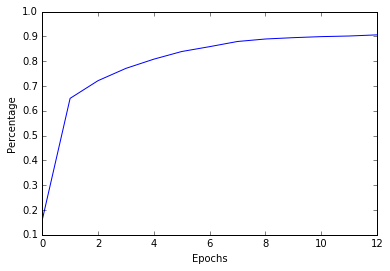
\includegraphics[width=0.4\textwidth]{acc_large.png}
\end{center}
\caption{Evolution of the Loss on held-out test data for the large feature vector}
\end{figure}

\noindent We then switched to using the genetic algorithm to improve on these two MLR as well as using the genetic algorithm without prior informed initialisation, in order to have a fair comparision. We also ran Q-learning with the two feature vectors.\\

\noindent The method of comparing the accuracy on "pro" moves will be used as the main method for testing the success of an algorithm. We will also present results on direct match-ups between the different AIs.
 
\subsection{Accuracy on Pro Moves}

\begin{figure}[H]
\begin{center}
    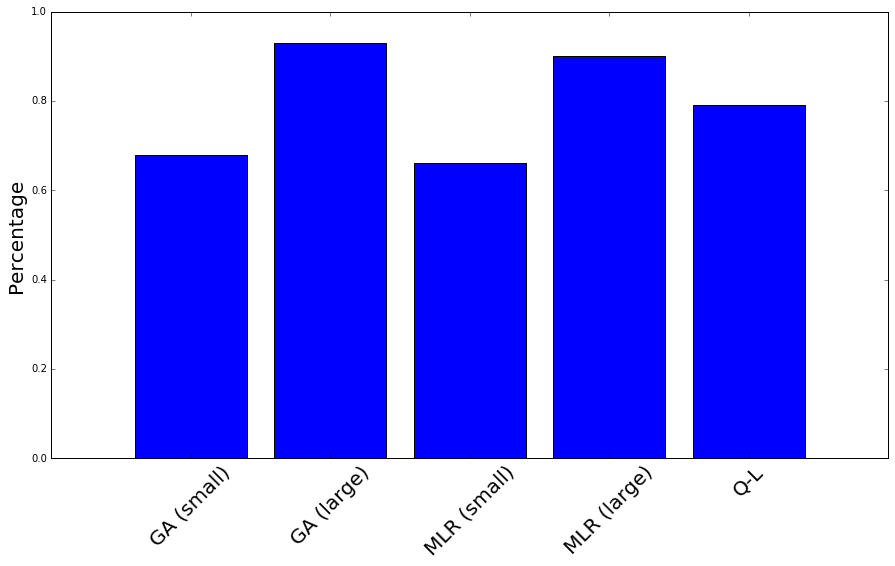
\includegraphics[width=0.4\textwidth]{acc.png}
\end{center}
\caption{Comparing accuracies of the different AIs}
\end{figure}
The key points of this figure are:
\begin{itemize}
\item larger feature vector yields better results than the smaller one, which would be expected. 
\item Genetic Algorithms increased the performance for both feature vectors
\item Q-learning reduced the performance
\end{itemize}

\subsection{One VS The Other}
\begin{table}[H]
\centering
\begin{tabular}{c|ccc|c|}
\cline{2-5}
                              & \multicolumn{1}{c|}{\textbf{GA (L)}} & \multicolumn{1}{c|}{\textbf{MLR (S)}} & \textbf{MLR (L)} & \textbf{Q-L} \\ \hline
\multicolumn{1}{|c|}{GA (S)}  & \multicolumn{1}{c|}{(8-15)}          & \multicolumn{1}{c|}{(15-5)}           & (15-6)           & (16-1)       \\ \hline
\multicolumn{1}{|c|}{GA (L)}  & \multicolumn{1}{c|}{}                & \multicolumn{1}{c|}{(15-0)}           & (16-0)           & (15-0)       \\ \cline{1-1} \cline{3-5} 
\multicolumn{1}{|c|}{MLR (S)} &                                      & \multicolumn{1}{c|}{}                 & (1-15)           & (8-15)       \\ \cline{1-1} \cline{4-5} 
\multicolumn{1}{|c|}{MLR (L)} &                                      &                                       &                  & (15-2)       \\ \cline{1-1} \cline{5-5} 
\end{tabular}
\caption{Match-up Results}
\end{table}

These results seemed for most of them in accordance with the accuracy results ! Genetically enhanced with large features is the best AI trained during this project !
 
\section{Discussion}

\subsection{Why did Q-Learning not work as expected?}

I ran into multiple issues with the Q-Learning part of this project. The first major issue was divergence. This was fixed by lowering drastically the learning rate as well as the discounting factor. The second issue I faced was that the Q-learning made the AI actually weaker. I did limit the impact by increasing the magnitude of the rewards but still did not manage to make the AI stronger with Q-learning. This is in my opinion due to fact that I was using a TD(0) algorithm whereas TD-Gammon uses $TD(\lambda)$. By using a longer path to update the weights, the system becomes much less sensitive to the stochastic nature of backgammon and the rolls of dice that could potentially changed the state of the game.

\subsection{Potential Improvements}

The next step would be to definitely switch from TD(0) to TD($\lambda$). Also I would also want to use a feed forward neural network as the evaluation function. Indeed, if the accuracy is extremely promising, I can still beat the AI myself (I am a decent player) because the trickiest moves, the AI still misses. A Neural Network should catch more of these !
\appendix

\section{System Description}

All the code is on github at: www.github.com/virgodi/pygammon.\\

\noindent You can play against the computer by typing: `python backgammon.py` in a terminal window !\\

\noindent Training and algorithms are contained in ipython notebooks in the folder notebooks\_and\_data


\bibliographystyle{plain} 
\bibliography{project-template}

\end{document}
